\chapter{Results and discussion}

\section{Performance of alternative optimizers}
We have tested performance of nougad using the seemingly promising ADAM optimizer, which has been shown to consistently perform well for variety of different problems. 

However, in the hyperparameter tuning stage it became clear that we won't be able to match or even approach performance of the momentum-based optimizer. The problem seems to lie in the fact that a combination of $\beta_1$ and $\beta_2$ decay factors for the first and second moment and $\alpha$ learning rate, that could provide fast enough convergence for ADAM optimizer to be competitive and practical to use, leads to under/overflows and produces \texttt{NaNs}. MSE produced by the best discovered parameter set fell short even when compared to OLS.

The surprisingly lackluster performance of ADAM optimizer compared to the momentum-based method leads us to believe that evaluating alternative optimizers could prove worthwhile.

\section{Quality of the artificial datasets}

In order to examine the overall structure of the generated data we used the R package EmbedSOM\footnote{\url{https://github.com/exaexa/EmbedSOM}}, that allows us to perform dimensional reduction via embedding the data into a 2D Self-Organizing Map (SOM) guided by Uniform Manifold Approximation and Projection (UMAP) generated landmarks: \cref{fig:SOM_tps}.

We were satisfied with the results as they seem to exhibit cluster separation and noise characteristics similar to real experimental data. It is also clear that our model works as expected and generates the predefined phenotypes correctly.

\begin{figure}
  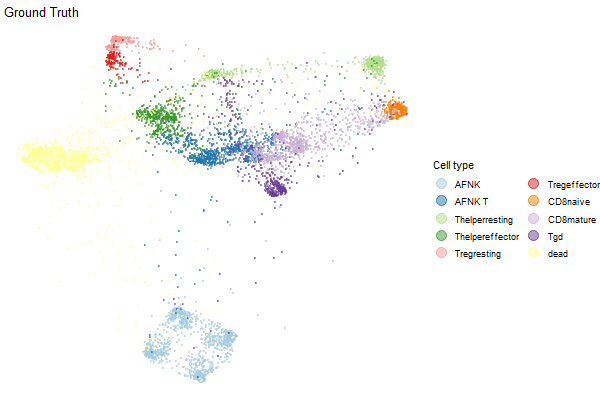
\includegraphics[width=1.0\linewidth]{img/SOM_types2.png}
  \caption{SOM embedding --- cell types in artificial data}
  \label{fig:SOM_tps}
\end{figure}

Among other manual evaluation methods we have also confirmed that our model is capable of emulating the spillover spreading artifact inherit to the process of acquisition of the real data: \cref{fig:spills}.

\begin{figure}
  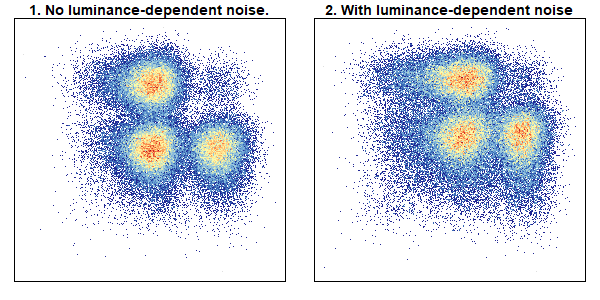
\includegraphics[width=1.0\linewidth]{img/spill.png}
  \caption{Spillover spreading simulated in the artificial data by adding fluorecent power dependent noise.}
  \label{fig:spills}
\end{figure}

\section{Quality of unmixing methods}
We are comparing three different size data sets mostly because different data size is more suitable for different types of visualizations. 
\begin{enumerate}
    \item \emph{Small data set} - $\text{size}=2002$ cells.
    \item \emph{Medium data set} - $\text{size}=10000$ cells.
    \item \emph{Big data set} - $\text{size}=100000$ cells.
\end{enumerate}

Size of the small data set is $2002$ even though the generator was passed $2000$ as the desired number of cells. This is because of previously discussed rounding - number of cells for each phenotype must be an integer. Exact sizes might change slightly if you rerun the script due to randomness.

Note that inverse hyperbolic sine transform\cite{asinh} is applied to all data sets in order to make visualizations and interpretation feasible: \cref{eq:asinh}.

\begin{equation}
\operatorname{arsinh} \frac{x}{100}=\ln (\frac{x}{100} + \sqrt{(\frac{x}{100})^2 + 1} 
\label{eq:asinh}
\end{equation}

The entire data generation and analysis pipeline is available as part of the supplemental materials.

\subsection{Comparison of MSE}

Mean squared errors for the testing data sets are illustrated in \cref{tab:MSEtb}.

\begin{table}[]
\begin{tabular}{lcccccc} \toprule 
\multirow{3}{*}{Method}  & \multicolumn{6}{c}{MSE}\\ 
\cmidrule(l{.5em}r{.5em}){2-7}
{}& \multicolumn{3}{c}{Unclamped}& \multicolumn{3}{c}{Clamped}\\
\cmidrule(l{.5em}r{.5em}){2-4}
\cmidrule(l{.5em}r{.5em}){5-7}
{} & small & medium & big  & small   & medium   & big\\
\midrule
\textbf{Nougad} & 0.5558  & 0.5452 & 0.5433 & \textcolor{red}{0.4942} & \textcolor{red}{0.4875}  & \textcolor{red}{0.4871}  \\
\textbf{WLS} & 2.1315 & 2.1795  & 2.1907  & 0.7752   & 0.7827 & 0.7833 \\
\textbf{OLS} & 1.9856  & 2.0197 & 2.0387  & 0.7337   & 0.7393 & 0.7417 \\
\bottomrule
\end{tabular}
\label{tab:MSEtb}
\caption{MSE on testing data sets across all methods.}
\end{table}

It is immediately obvious how much does simply clamping the results to zero help for OLS and WLS methods and while it helps for Nougad the difference is rather small. This does however, make some sense. There is no such thing as negative expression but OLS and WLS do not have any non negative constraints therefore shifting the negative results to zero must decrease the error. Same thing applies for Nougad however since this algorithm is already heavily biased towards positive results thanks to high \param{nw} parameter the difference is rather small. 

Nougad clearly comes out on top in this comparison. However, OLS performs quite well when clamped to zero and we could say it gets close to Nougad while WLS performs the worst out of the three, both clamped and unclamped.

Hypothesis testing using squared error was done to verify than Nougad outperforms both competing methods (clamped and unclamped) with statisticall significance.

\subsection{Distribution of errors in the result}
Calculated and visualized on big data set.


In this section we examine the distribution of squared errors across the entire data set. Since this is per element error even the smallest data set is almost too large for this visualization giving us $2002\cdot21=42042$ points. 

From \cref{fig:SE_auc} is evident that when we are comparing the unclamped results there is no contest Nougad clearly performs the best.

\begin{figure}
  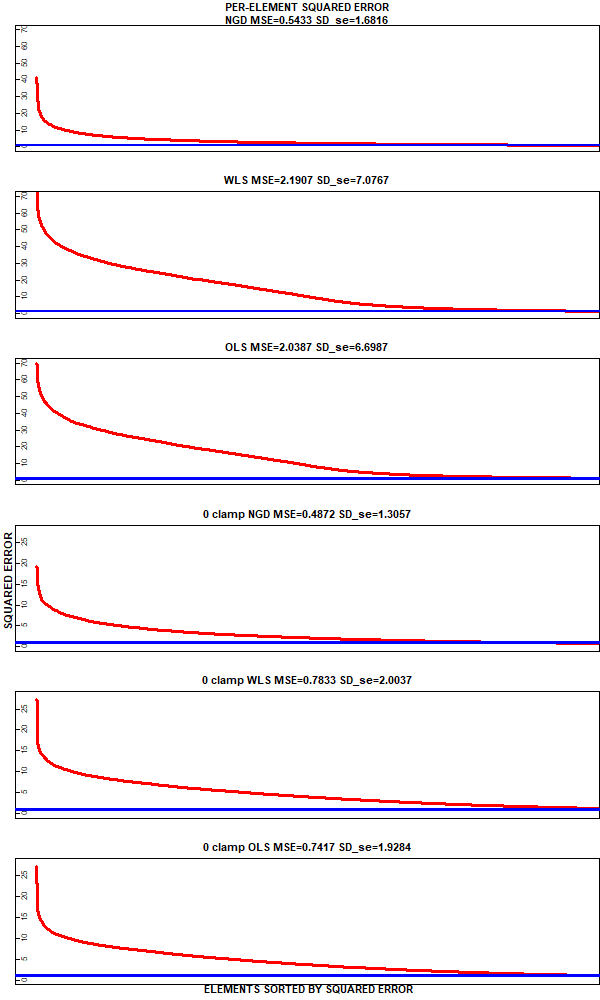
\includegraphics[width=0.9\linewidth]{img/SE_auc.png}
  \caption{Per-element squared error for individual data sets sorted from highest --- blue line represents SE=1.}
  \label{fig:SE_auc}
\end{figure}

Clamping the methods results in significantly reduced error especially for OLS and WLS. What is quite interesting is that the top error percentile has decreased significantly for both linear methods as well. This suggests that the biggest errors produced by these methods stem from negative abundances. Still Nougad remains in the even compared to clamped OLS.

\subsection{Per-cell mean squared error distribution}

Calculated on big data set, visualized on small data set.

This comparison focuses on per-cell MSE represented by the red line, while the green line denotes relative luminance of the given cell. Vertical labels for cell types are also added: \cref{fig:MSEcell_dist}.

When unclamped similarly to the previous sections Nougad is clearly superior to both OLS and WLS. It is interesting to note that while there seems to be a degree of correlation between cell luminance and absolute MSE value, it does not appear as strong as we would perhaps expect and seems even weaker in the data unmixed by Nougad compared to the other two methods.

\begin{figure}
  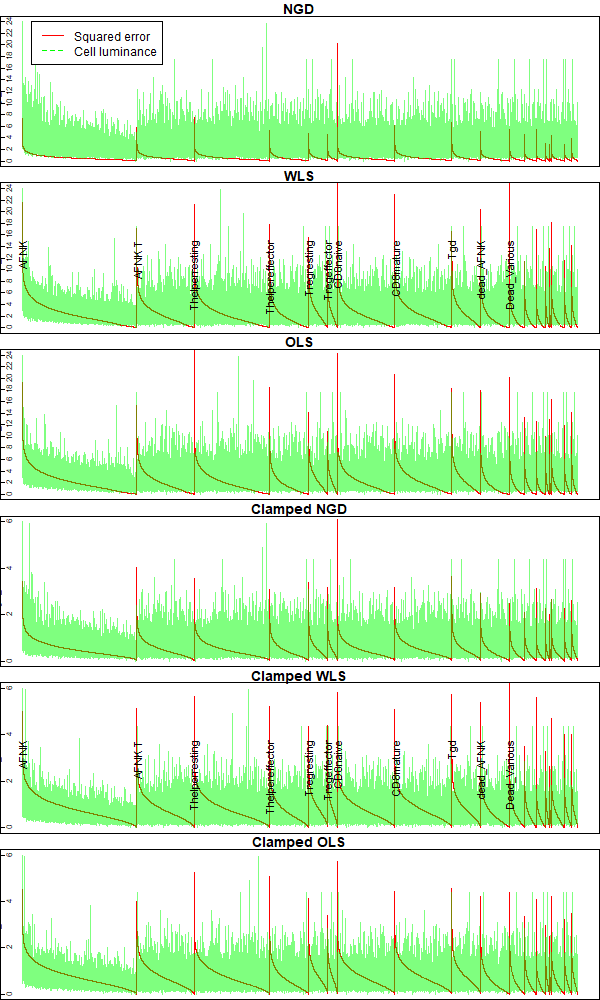
\includegraphics[width=1.0\linewidth]{img/errdist.png}
  \caption{Per-cell MSE distribution using unclamped methods}
  \label{fig:MSEcell_dist}
\end{figure}

After clamping the methods we can see that OLS performs much closer to Nougad, but Nougad still retains the overall advantage.

\subsection{Correlation of unmixing error with cell luminance}

The idea behind this metric is that the better the unmixing method is, the more it should avoid increasing the absolute error proportionally to the cell luminance.  

Nougad shows significantly lower correlation than other methods both clamped and unclamped: \cref{fig:bright_cell_cor}. Correlation for nougad could be condidered borderline weak while for other methods it lies firmly in the moderate territory\cite{cor2018}. This suggests that nougad is better equipped to deal with the luminance-dependent noise.

\begin{figure}
  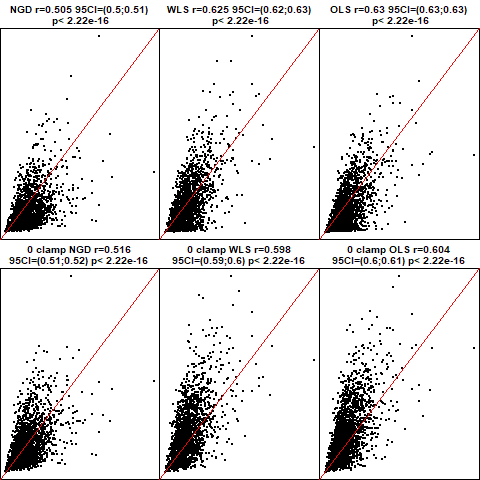
\includegraphics[width=0.8\linewidth]{img/lumcorr.png}
  \caption{Correlation of per-cell MSE with cell luminance}
  \label{fig:bright_cell_cor}
\end{figure}

\subsection{Error distribution in individual dimensions}


This metric focuses on unmixing performance over individual spectra.

On per-spectrum basis there are some instances where the difference betwenn nougad and investigated linear methods is quite small. One such case is the spectrum for the CD4 marker when unmixing using clamped methods : \cref{fig:hists}(b). However, even though the performance of clamped linear methods can get quite close to that of nougad, this is more of an exception than a rule. Overall nougad outperforms both OLS and WLS across most of the spectra.


\begin{figure}
  \centering
  \subfloat[][]{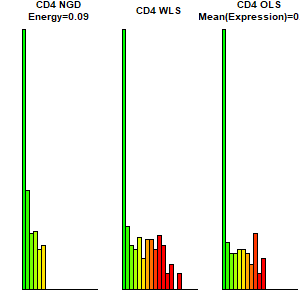
\includegraphics[width=.45\linewidth]{img/CD4.png}}\quad
  \subfloat[][]{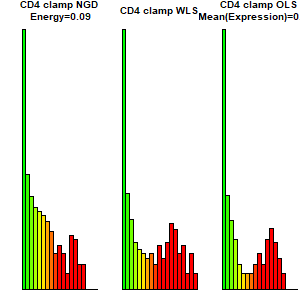
\includegraphics[width=.45\linewidth]{img/CD4_clp.png}}\\
  \subfloat[][]{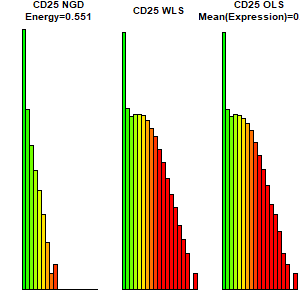
\includegraphics[width=.45\linewidth]{img/CD25.png}}\quad
  \subfloat[][]{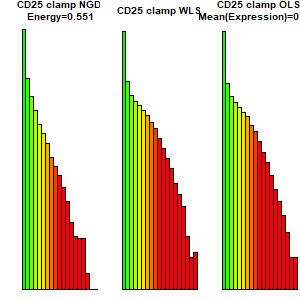
\includegraphics[width=.45\linewidth]{img/CD25_clp.png}}
  \caption{Histograms of per-cell MSEs for CD4 and CD25 antigens. Caution --- bin width and x limits differ between clamped and unclamped methods!}
  \label{fig:hists}
\end{figure}

It is important to highlight that the X axis limits and therefore bin width differ between clamped and unclamped comparisons which means that we cannot directly cross-compare the two. However, relative comparisons are of course completely valid.

Also note that the histograms are log-scaled and the first bin is always clipped.

This metric was calculated and visualized on the big data set. Histograms for all remaining spectra can be found in the supplement.

\subsubsection{Per-spectrum MSE correlation with luminance}

Intuitively we would expect higher error in dimmer spectra but the analysis is inconclusive as confidence intervals are too wide and there is no statistically significant difference between methods.

Calculation performed on the big data set with exact results including $95\%$ CIs and p-values can be found in the supplement.

\subsubsection{Per-spectrum mean error correlation with average expression}

Our analysis supports the hypothesis that mean per-spectrum SE is inversely correlated with mean expression. The results suggest medium to strong inverse correlation across all methods clamped and unclamped. Confidence intervals are very wide therefore, there is no statistically significant difference between individual methods.

Calculation performed on the big data set with exact results including $95\%$ CIs and p-values can be found in the supplement.

\section{Observing the detailed errors on dot-plots}

This comparison gives more insight into how much is the cell's position in some of the sub-spaces given by spectra pairs affected by errors.

Black points represent the ground truth --- cell's original location in the selected 2D subspace while red lines are drawn from this point to the location of the same cell in the unmixing result for the examined method. This metric is visualized on the big data set.

Looking at some of the markers the difference can be quite small even in unclamped methods as demonstrated in \cref{fig:bld}(b), where it could even be argued that OLS slightly outperforms nougad. However, this is again more of an exception as nougad has a clear advantage in most other, both stronger and weaker markers, as exhibited in \cref{fig:bld}(a,c,d). An argument could be made for OLS outperforming WLS.

\begin{figure}
  \centering
  \subfloat[][]{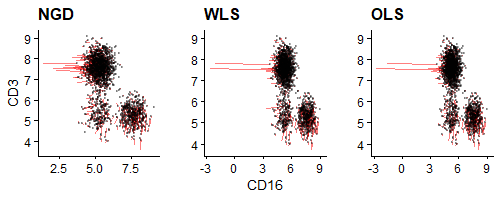
\includegraphics[width=0.7\linewidth]{img/blood_CD16xCD3_nocl.png}}\\
  \subfloat[][]{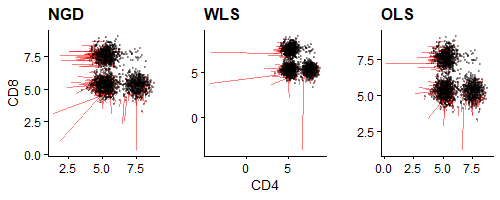
\includegraphics[width=0.7\linewidth]{img/blood_CD4xCD8_nocl.png}}\\
  \subfloat[][]{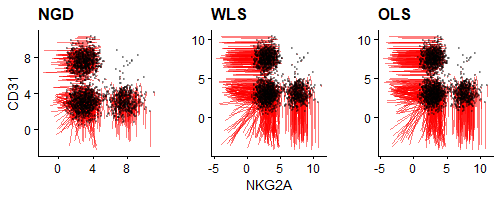
\includegraphics[width=0.7\linewidth]{img/blood_NKG2AxCD31_nocl.png}}\\
  \subfloat[][]{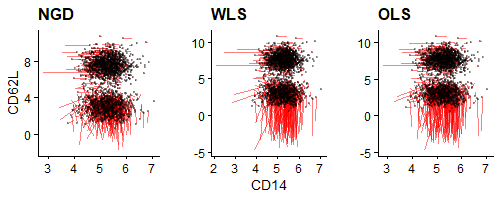
\includegraphics[width=0.7\linewidth]{img/blood_CD14xCD62L_nocl.png}}
  \caption{2D plots on selected markers for unclamped methods.}
  \label{fig:bld}
\end{figure}




\begin{figure}
  \centering
  \subfloat[][]{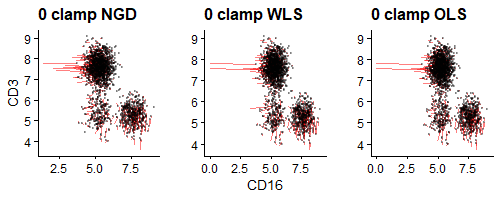
\includegraphics[width=0.7\linewidth]{img/bloodCD16xCD3_cl.png}}\\
  \subfloat[][]{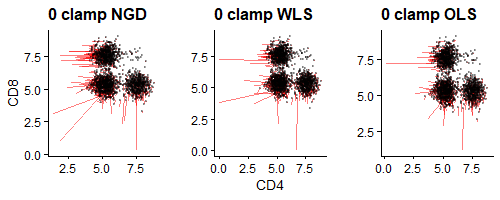
\includegraphics[width=0.7\linewidth]{img/bloodCD4xCD8_cl.png}}\\
  \subfloat[][]{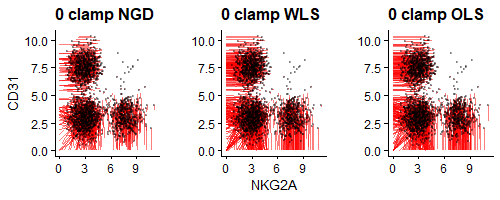
\includegraphics[width=0.7\linewidth]{img/bloodNKG2AxCD31_cl.png}}\\
  \subfloat[][]{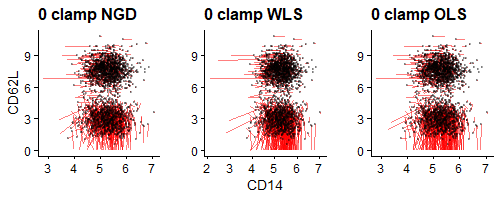
\includegraphics[width=0.7\linewidth]{img/bloodCD14xCD62L_cl.png}}
  \caption{2D plots on selected markers for clamped methods.}
  \label{fig:bld_cl}
\end{figure}

When we examine the clamped methods, OLS, WLS and nougad seem to trade blows more often than previously. However, nougad still wins in most comparisons \cref{fig:bld_cl}.

We have prepared another type of visualization for the same data --- plotting the ground truth and unmixing results for each of the three methods as separate plots and color the points by the severity of the error.

This type of visualization helps to emphasize the fact that the majority of the more severe errors tends to happen in the weaker markers.

Main advantage of Nougad is well illustrated in \cref{fig:blob_noclp} and \cref{fig:blob_clp} where we can see that just clamping the method and effectively putting all negative points onto an axis is not an optimal solution and even though the difference in error might not be that big the way Nougad deals with such situations is clearly superior. 

\begin{figure}
  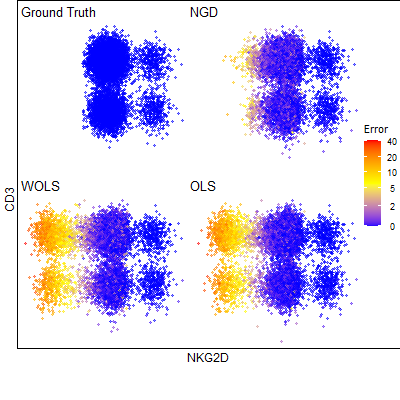
\includegraphics[width=0.7\linewidth]{img/blobs_noclp.png}
  \caption{2D error color plot NKG2D$\times$CD3 unclamped}
  \label{fig:blob_noclp}
\end{figure}

\begin{figure}
  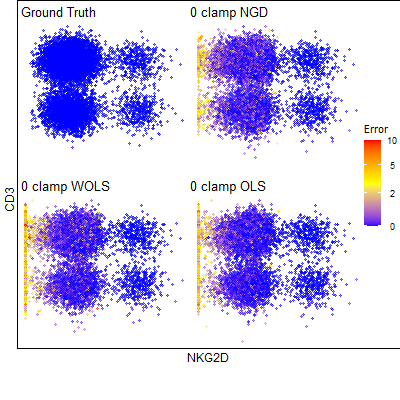
\includegraphics[width=0.7\linewidth]{img/blobs_clp.png}
  \caption{2D error color plot NKG2D$\times$CD3 clamped}
  \label{fig:blob_clp}
\end{figure}

2D plots of both types for all unique spectra are available in the supplement. 

\section{Error overview using dimensionality reduction}
In order to further examine the per-cell error characteristics in all dimensions we used the previously generated UMAP guided SOM from \cref{fig:SOM_tps} for 2D visualization. Unmixing results for the evaluated methods are embedded into the SOM and colored by per-cell MSE.

As evident from \cref{fig:SOM_noclp} Nougad takes a comfortable lead against unclamped methods. 

\begin{figure}
  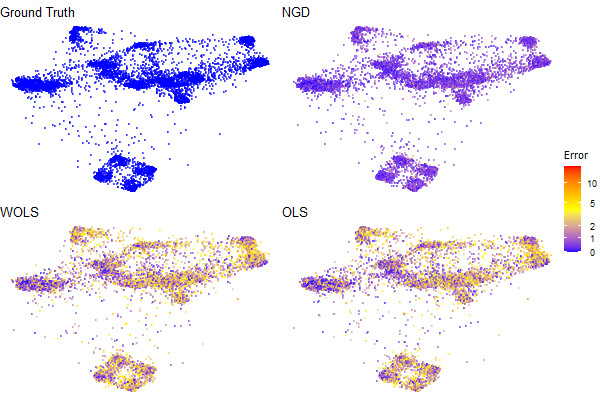
\includegraphics[width=1.0\linewidth]{img/SOM_err_noclp2.png}
  \caption{SOM embedding colored by MSE unclamped}
  \label{fig:SOM_noclp}
\end{figure}

When clamped the differences between Nougad and OLS become much harder to spot as they are practically interchangeable: \cref{fig:SOM_clp}. 

\begin{figure}
  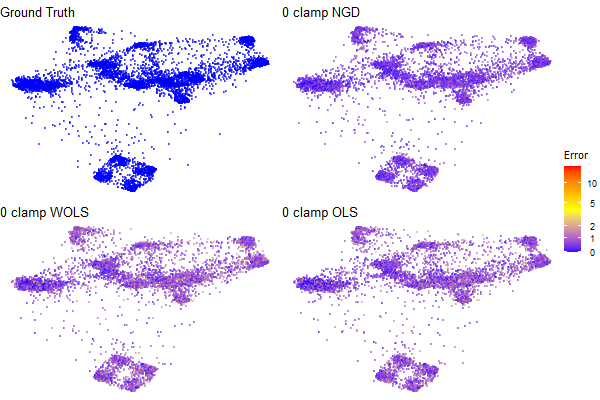
\includegraphics[width=1.0\linewidth]{img/SOM_err_clp2.png}
  \caption{SOM embedding colored by MSE clamped}
  \label{fig:SOM_clp}
\end{figure}

Finally we can take a look at the different unmixing methods and their comparison to ground truth using the `blood plots'. Do note that we did have to increase expression based and luminance based noise when generating the data for this visualization in order to make the differences more apparent to the reader. Arguably this is more true to life, since real data do tend to be quite noisy. 

\begin{figure}
  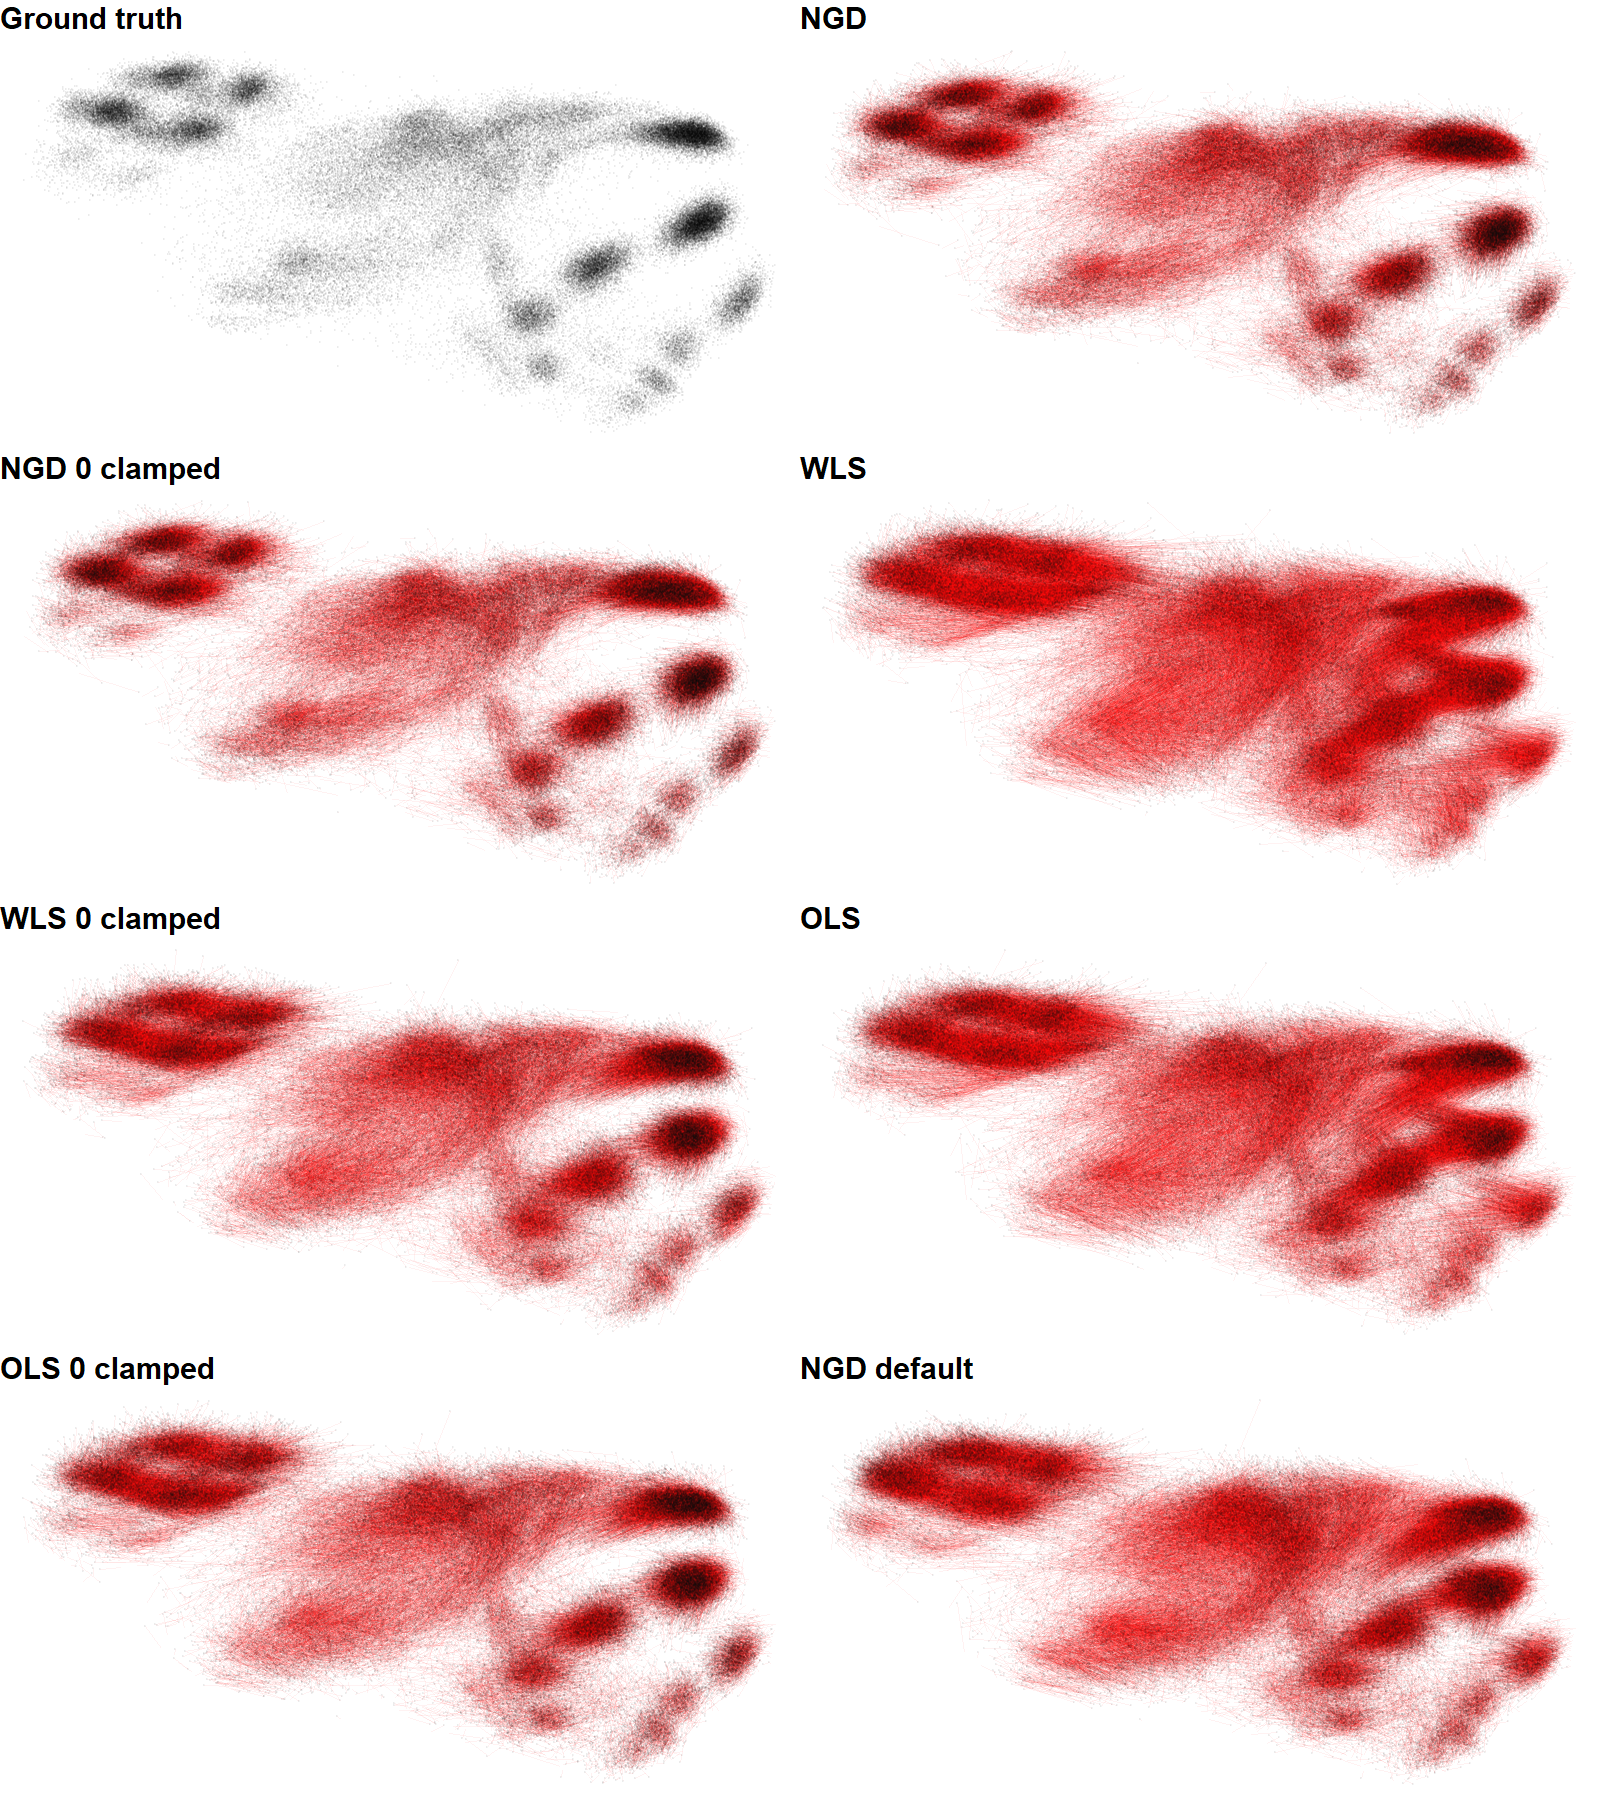
\includegraphics[width=1\linewidth]{img/8-way.png}
  \caption{Error comparison for investigated unmixing methods in 2D using SOM embedding.}
  \label{fig:8-way}
\end{figure}

Note that in \cref{fig:8-way} we are using `inverse blood plots' --- the black/grey points are drawn in the location of unmixed data and red lines are drawn from those points towards the ground truth location. This is done to improve readability and make easier for the reader to spot the differences. That said, this plot can be interpreted in a similar way as previous blood plots --- more red lines means more errors. This comparison clearly shows that Nougad performs the best with previously established hierarchy for the remaining methods. Nougad tends to most faithfully retain the cluster separation which is a challenge for all other methods and while clamped OLS gets somewhat close the difference is still clear. We also choose this visualization to demonstrate that hyperparameter tuning clearly matters --- Nougad with default parameters performs somewhat similarly to clamped WLS, meaning clearly better than unclamped WLS and OLS and clearly worse than clamped OLS and therefore significantly worse than Nougad with optimized hyperparameters.
Size of both data sets used for visualization was $\sim$100 000.

\section{Results on real-world datasets}
While we cannot evaluate how well the different methods perform on a real data set, since the ground truth is not known, we can still do a relative comparison and comment on the differences.

\begin{figure}
  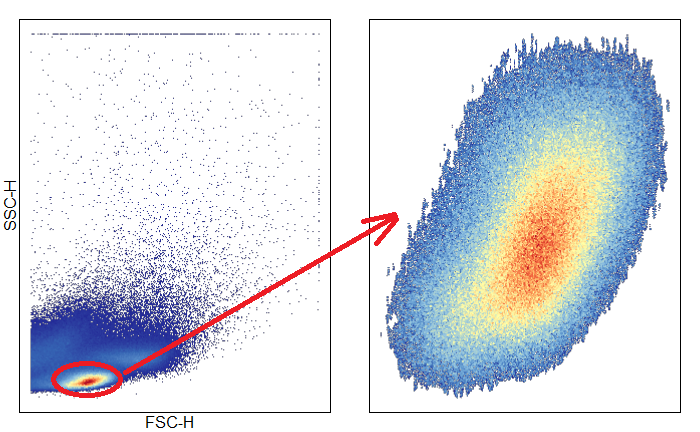
\includegraphics[width=1\linewidth]{img/my_gate.png}
  \caption{Isolating Lymphocytes from the experimental data set using density-based gating approach (Lymphocyte population circled red).}
  \label{fig:my_gate}
\end{figure}


We will limit our comparison to Lymphocytes to remain consistent with the artificial data. Our gating strategy is visualized in \cref{fig:my_gate}. Note that we decided to forgo the more traditional manual gating strategy in favor of density-based gating using k-nearest neighbors algorithm that allows us to isolate high density regions and their neighborhood (implementation available in the supplement).

In \cref{fig:6-way_nb} we can see how the spatial organization of real data looks after unmixing when embedded --- the data is colored using selected markers.

There are no truly objective conclusions to be drawn here. Only thing we can be fairly certain about is that relative differences between methods are somewhat consistent with the artificial data. Nougad in both its variations is the most dissimilar to the other methods while its variants seem quite close to each other. Both OLS and WLS differ quite a bit between their clamped and unclamped versions and we could argue that OLS in its clamped variation is the least dissimilar to Nougad out of all OLS and WLS variants. Note that due to the nature of the algorithm used for embedding and plot generation there is no good way to force the same orientation of the resulting maps however it should be fairly obvious which clusters correspond to each other in maps for different methods.

We must stress that this comparison is purely empirical and somewhat subjective therefore it should not be used to draw any conclusions about the performance of these algorithms.

\begin{figure}
  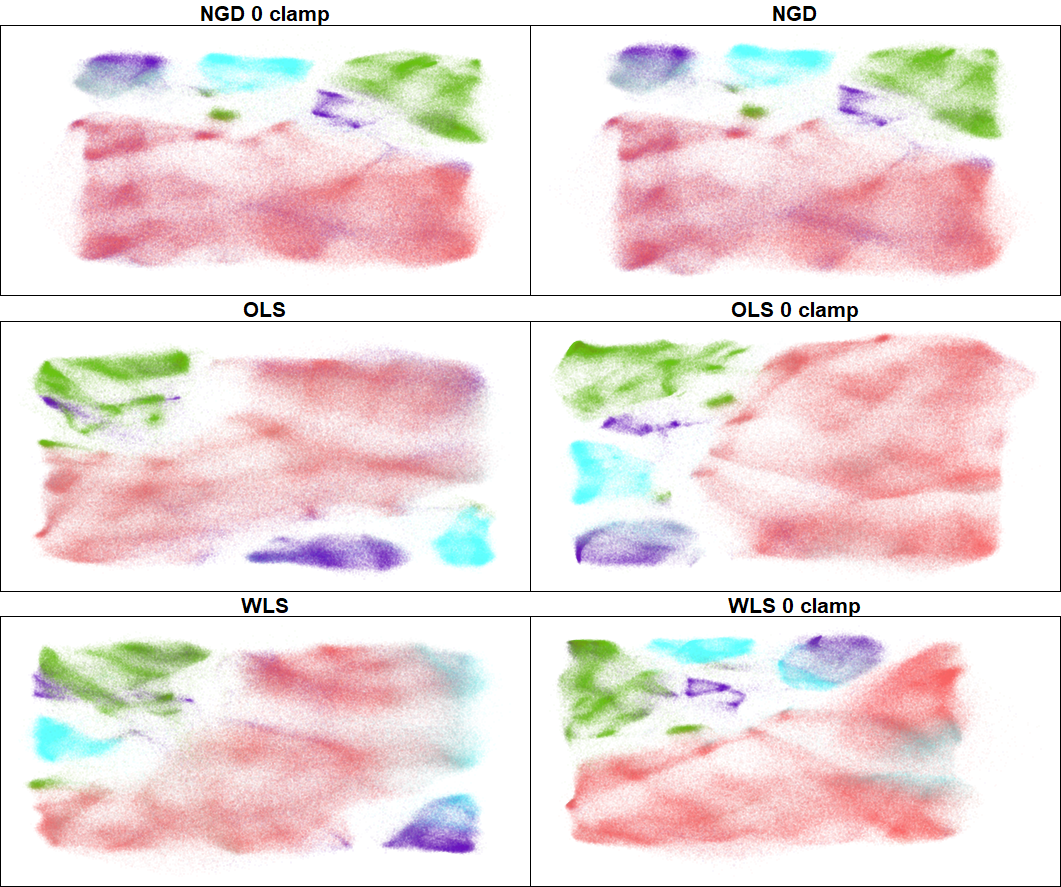
\includegraphics[width=1\linewidth]{img/6way_asinh1000v2.png}
  \caption{Real data unmixed via tested methods visualized in 2D using SOM embedding. Colored by selected markers --- CD4 (red), CD8 (green), CD16 (cyan) and gdTCR (blue).}
  \label{fig:6-way_nb}
\end{figure}

\section{Discussion}
We have found that for our simulated data Nougad algorithm consistently performs better than OLS and WLS alternatives, both clamped and unclamped. While there is a possibility than in some instances in low-error regions Nougad could be outperformed by clamped OLS, this is more of an exception than a rule. Furthemore, in medium or high-error regions Nougad, even in its unclamped variation, significantly outperforms clamped OLS. In our opinion potentially getting slightly more noise in a low-error region seems like a worthwhile trade-off for consistently better handling of more challenging regions.  

Results show that for the tested artificial data Nougad is the better choice. 

The validity of the simulated data cannot be entirely proven however, it should be sufficient for the evaluation of unmixing performance.

Objective performance evalution for different unmixing methods is not possible on real experimental data which is why we do not consider provided real data comparisons to be evaluation metrics. We do however make an argument that the relative differences between the methods seem to hold even in real data.

Ultimately our testing is limited --- we cannot guarantee same performance across all possible experiment types, hardware configurations and other variables. On the other hand there is nothing that would lead us to believe that Nougad should fail for data with different characteristics (within reason of course). Another limitation is the reliance on optimized hyperparameters --- it is possible that for significantly different combinations of fluorochromes and detectors the optimal hyperparameters will differ. Of course since our tuning process is well documented and reproducible it is possible to replicate it for different conditions. 

As a result we do believe that Nougad provides a viable and likely superior alternative to OLS and WLS for unmixing of spectral flow cytometry data, especially for those who would like to avoid using `black box' and usually paid software provided by different private companies. We would therefore recommend considering Nougad as unmixing algorithm of choice to scientists who value maximum reproducibility and transparency for their experiments.